\documentclass{beamer}
\usepackage{geometry}
\usepackage{graphicx, dblfloatfix}
\usepackage{amsmath, amssymb, amsfonts}

\title{Gamma Cross Sections}
\author{Aman LaChapelle}
\institute{University of Chicago}
\date{October 21, 2015}

\AtBeginSection[]
{
  \begin{frame}
    \frametitle{Table of Contents}
    \tableofcontents[currentsection]
  \end{frame}
}

\begin{document}

\frame{
	\titlepage
}

\frame{
	\frametitle{Gamma Cross Sections}
	\begin{itemize}
		\item Analyzing the Data
		\item Issues encountered in Analysis
		\item Resolution
		\item References
	\end{itemize}
	The general theory of each step will be interspersed throughout.
}

\section{Analyzing the Data}
	\frame{  %switch up this one and the next one?
		\frametitle{Gaussian Fits to Data}
		\begin{figure}[!htb]
			\centering
			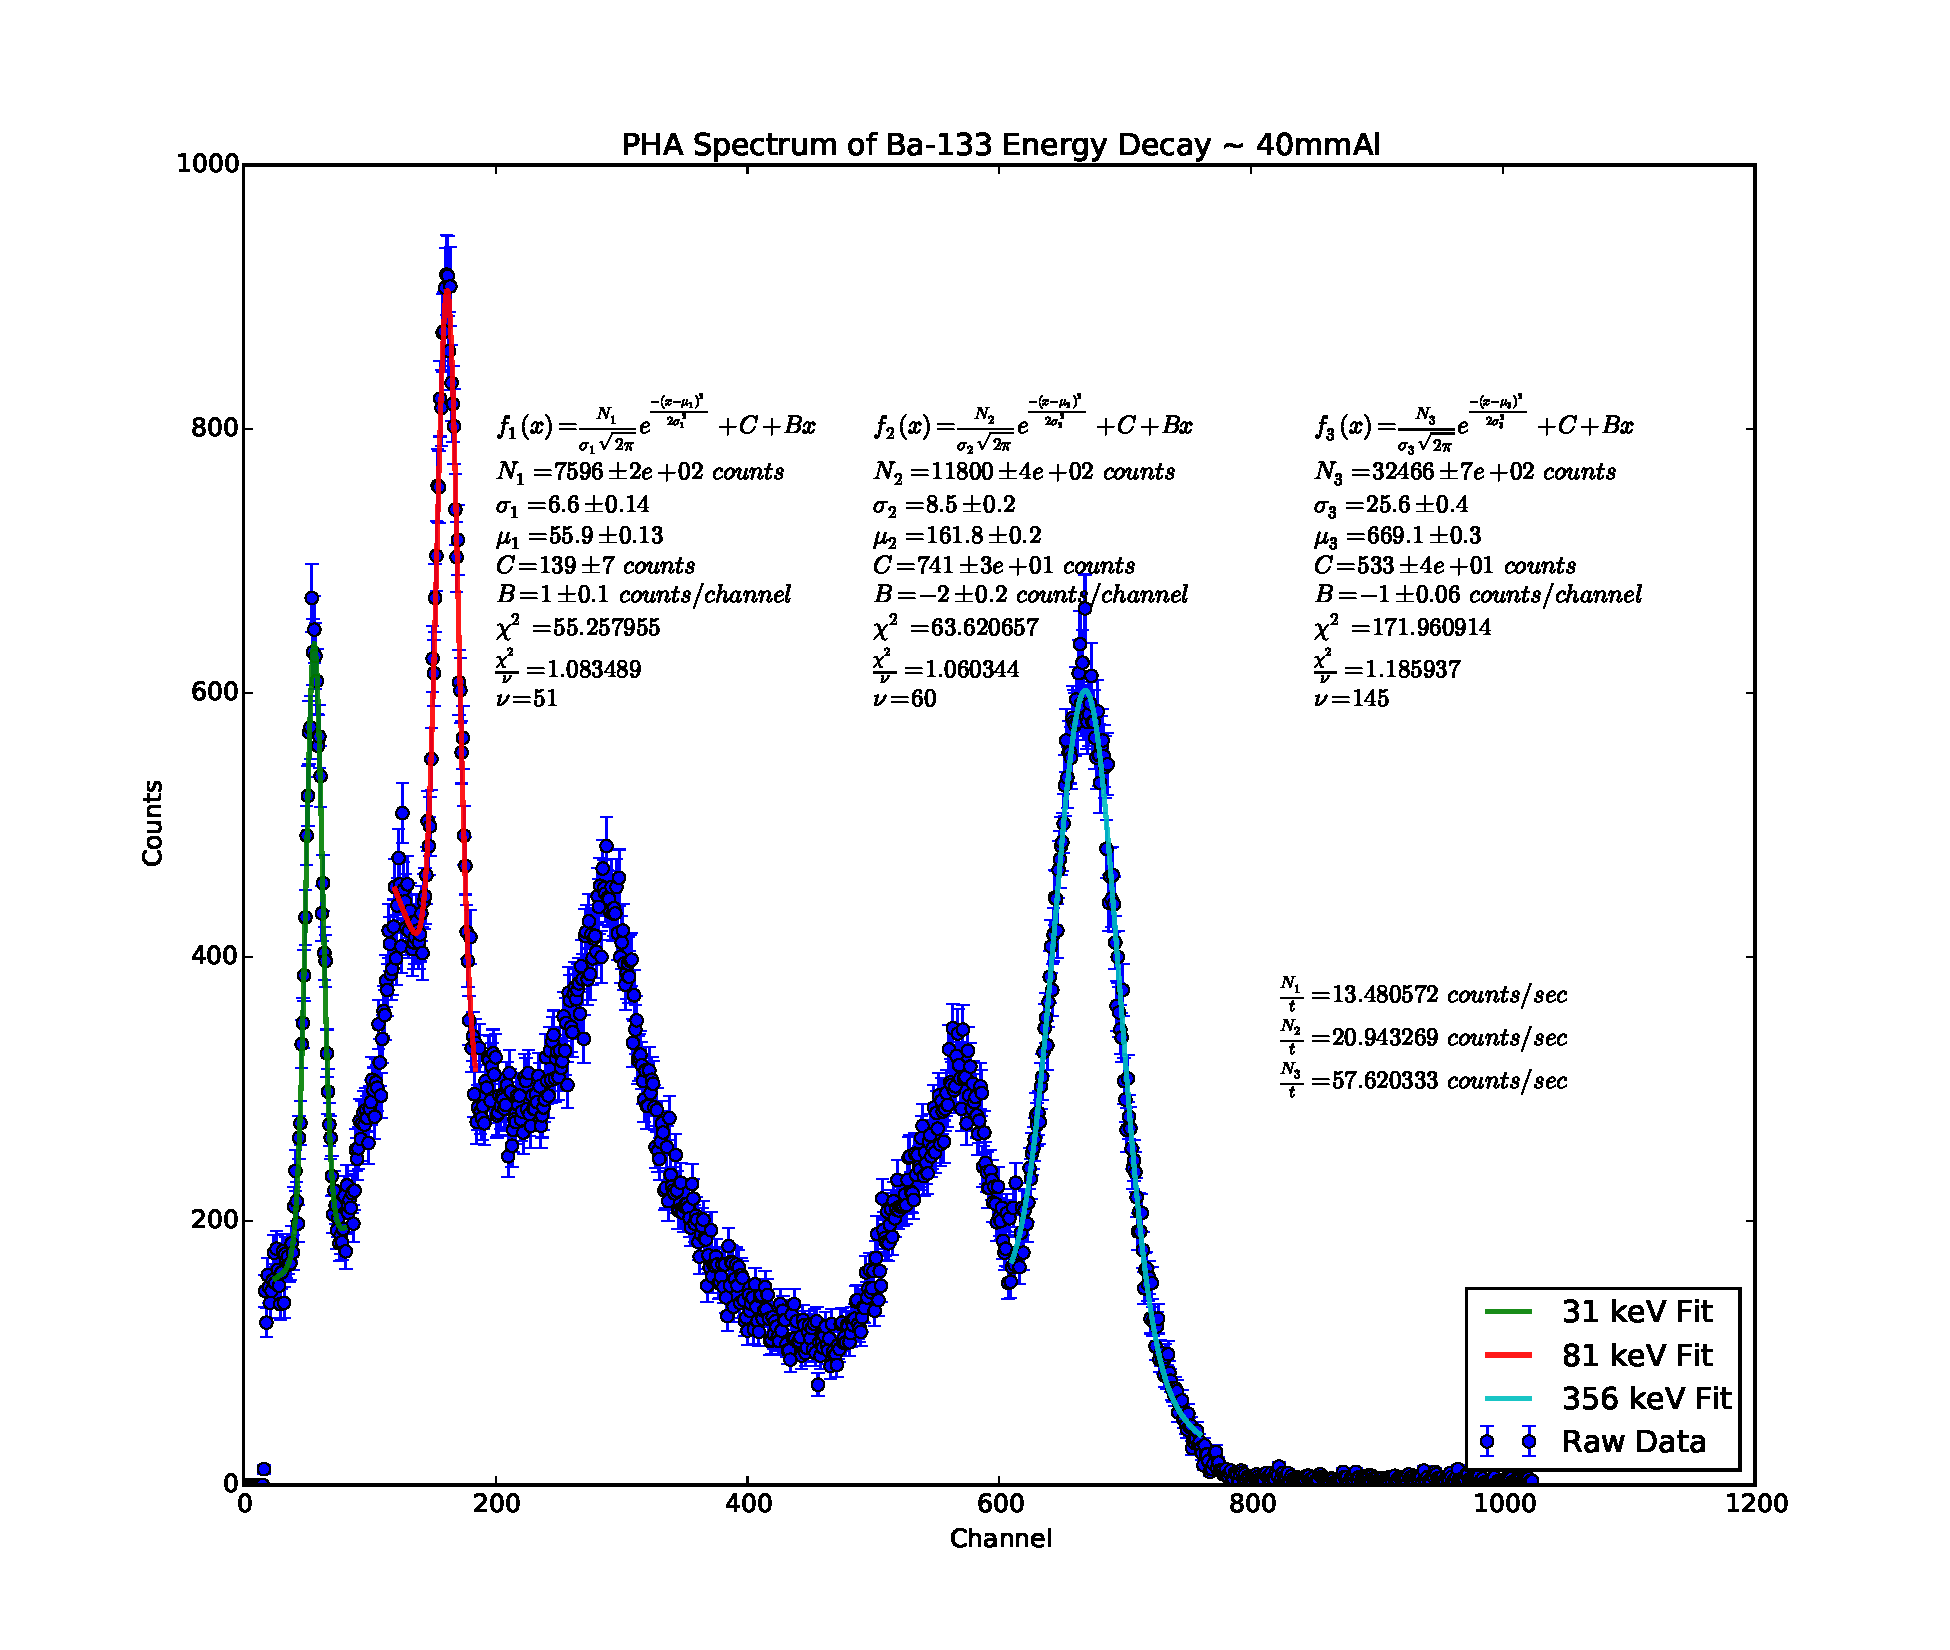
\includegraphics[height=6cm]{../plots/Ba40mmAl.pdf}
		\end{figure}
		Notes:
		\begin{itemize}
			\item Notice the fit function - linear background
			\item $\tilde{\chi}^2$ - gives confidence in the form of the fit as well as the fit itself
		\end{itemize}
	}
	\frame{
		\frametitle{Gaussian Fits to Data}
		Fit Function:
		\begin{equation*}
			f(x) = \frac{N}{\sigma\sqrt{2\pi}} e^{ \frac{-(x-\mu)^2}{2\sigma^2} } + Ax + B
		\end{equation*}
		\begin{itemize}
			\item Linear background is not a rate in time; it's a rate over the channels
			\item $\implies$ Background measures:
			\begin{itemize}
				\item susceptibility (to noise) by channel - $A$
				\item overall susceptibility (to noise)  - $B$
			\end{itemize}
			\item We assume that this noise is random and is not caused by our apparatus
			\begin{itemize}
				\item $\implies$ It comes from another source(s)
			\end{itemize}
			\item Why aren't they delta functions?
			\begin{itemize}
				\item energies are one value, width comes from detector
			\end{itemize}
		\end{itemize}
	}
	\frame{
		\frametitle{Gaussian Fits to Data}
		\begin{figure}[!htb]
			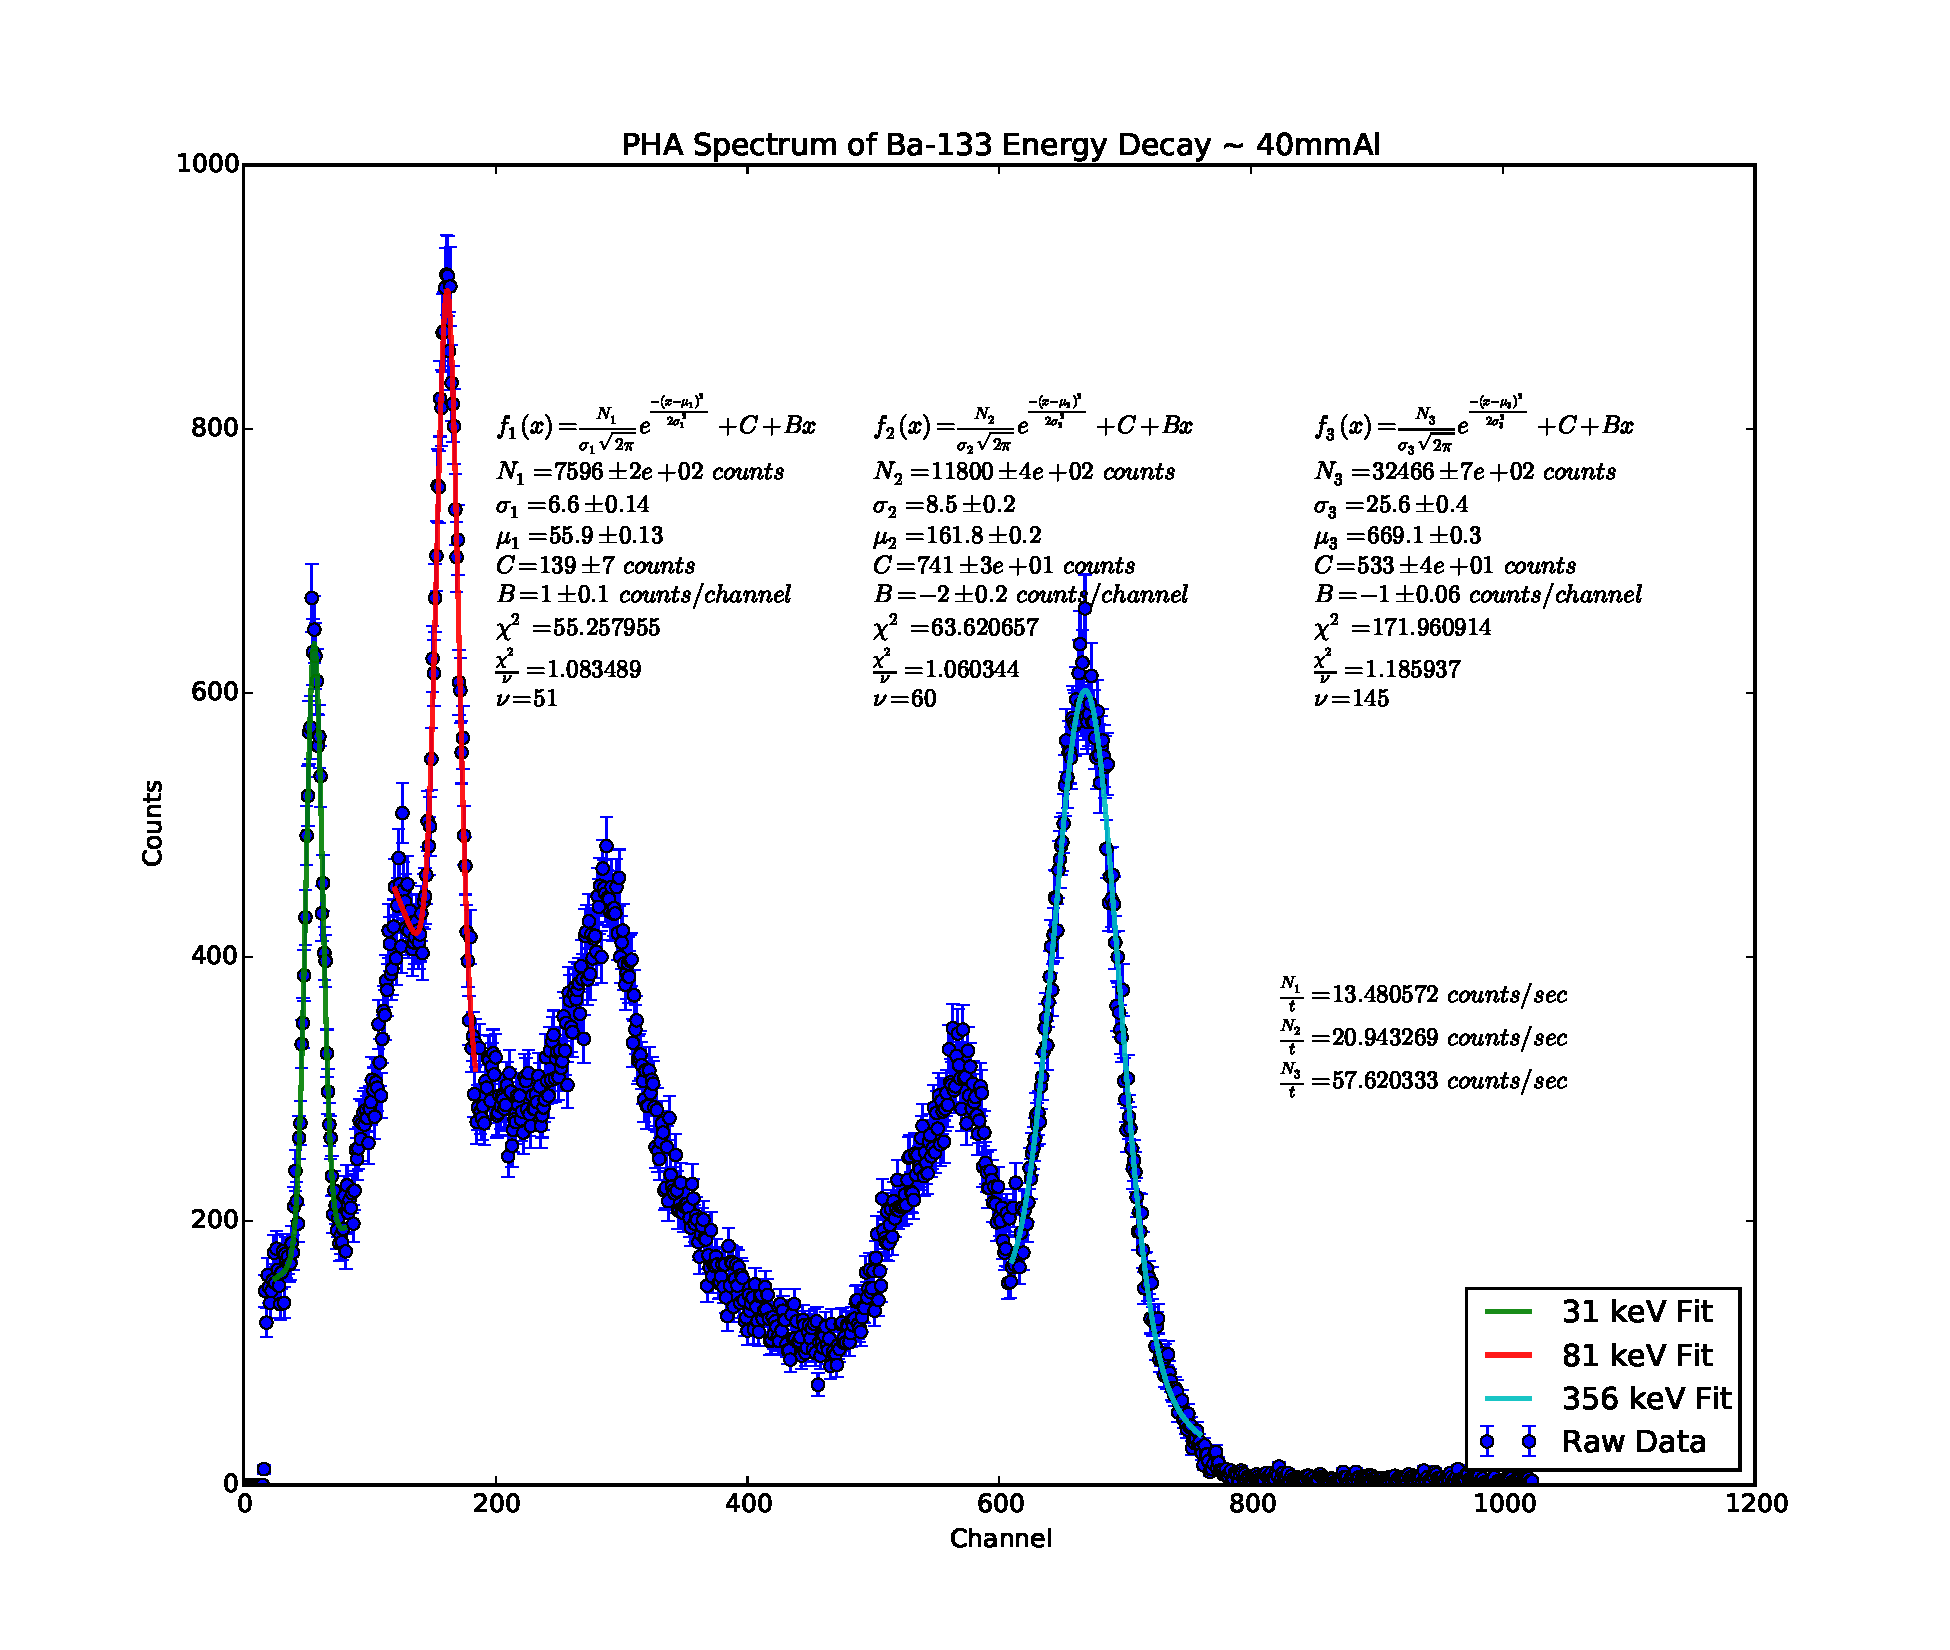
\includegraphics[scale=.1]{../plots/Ba40mmAl.pdf}
		\end{figure}
		Then what are these other peaks?
		\begin{itemize}
			\item Compton Edge and Backscatter
			\begin{itemize}
				\item Peak energies are known - ignore these other features$^\dagger$
			\end{itemize}
		\end{itemize}
		\hspace{1cm}
		\begin{flushleft}
		\tiny{$^\dagger$We should never ignore features, but once we verify that we aren't interested in them we can effectively ignore them.}
		\end{flushleft}
	}
	\frame{
		\frametitle{Fitting to Find Countrates}
		\begin{figure}[!htb]
			\centering
			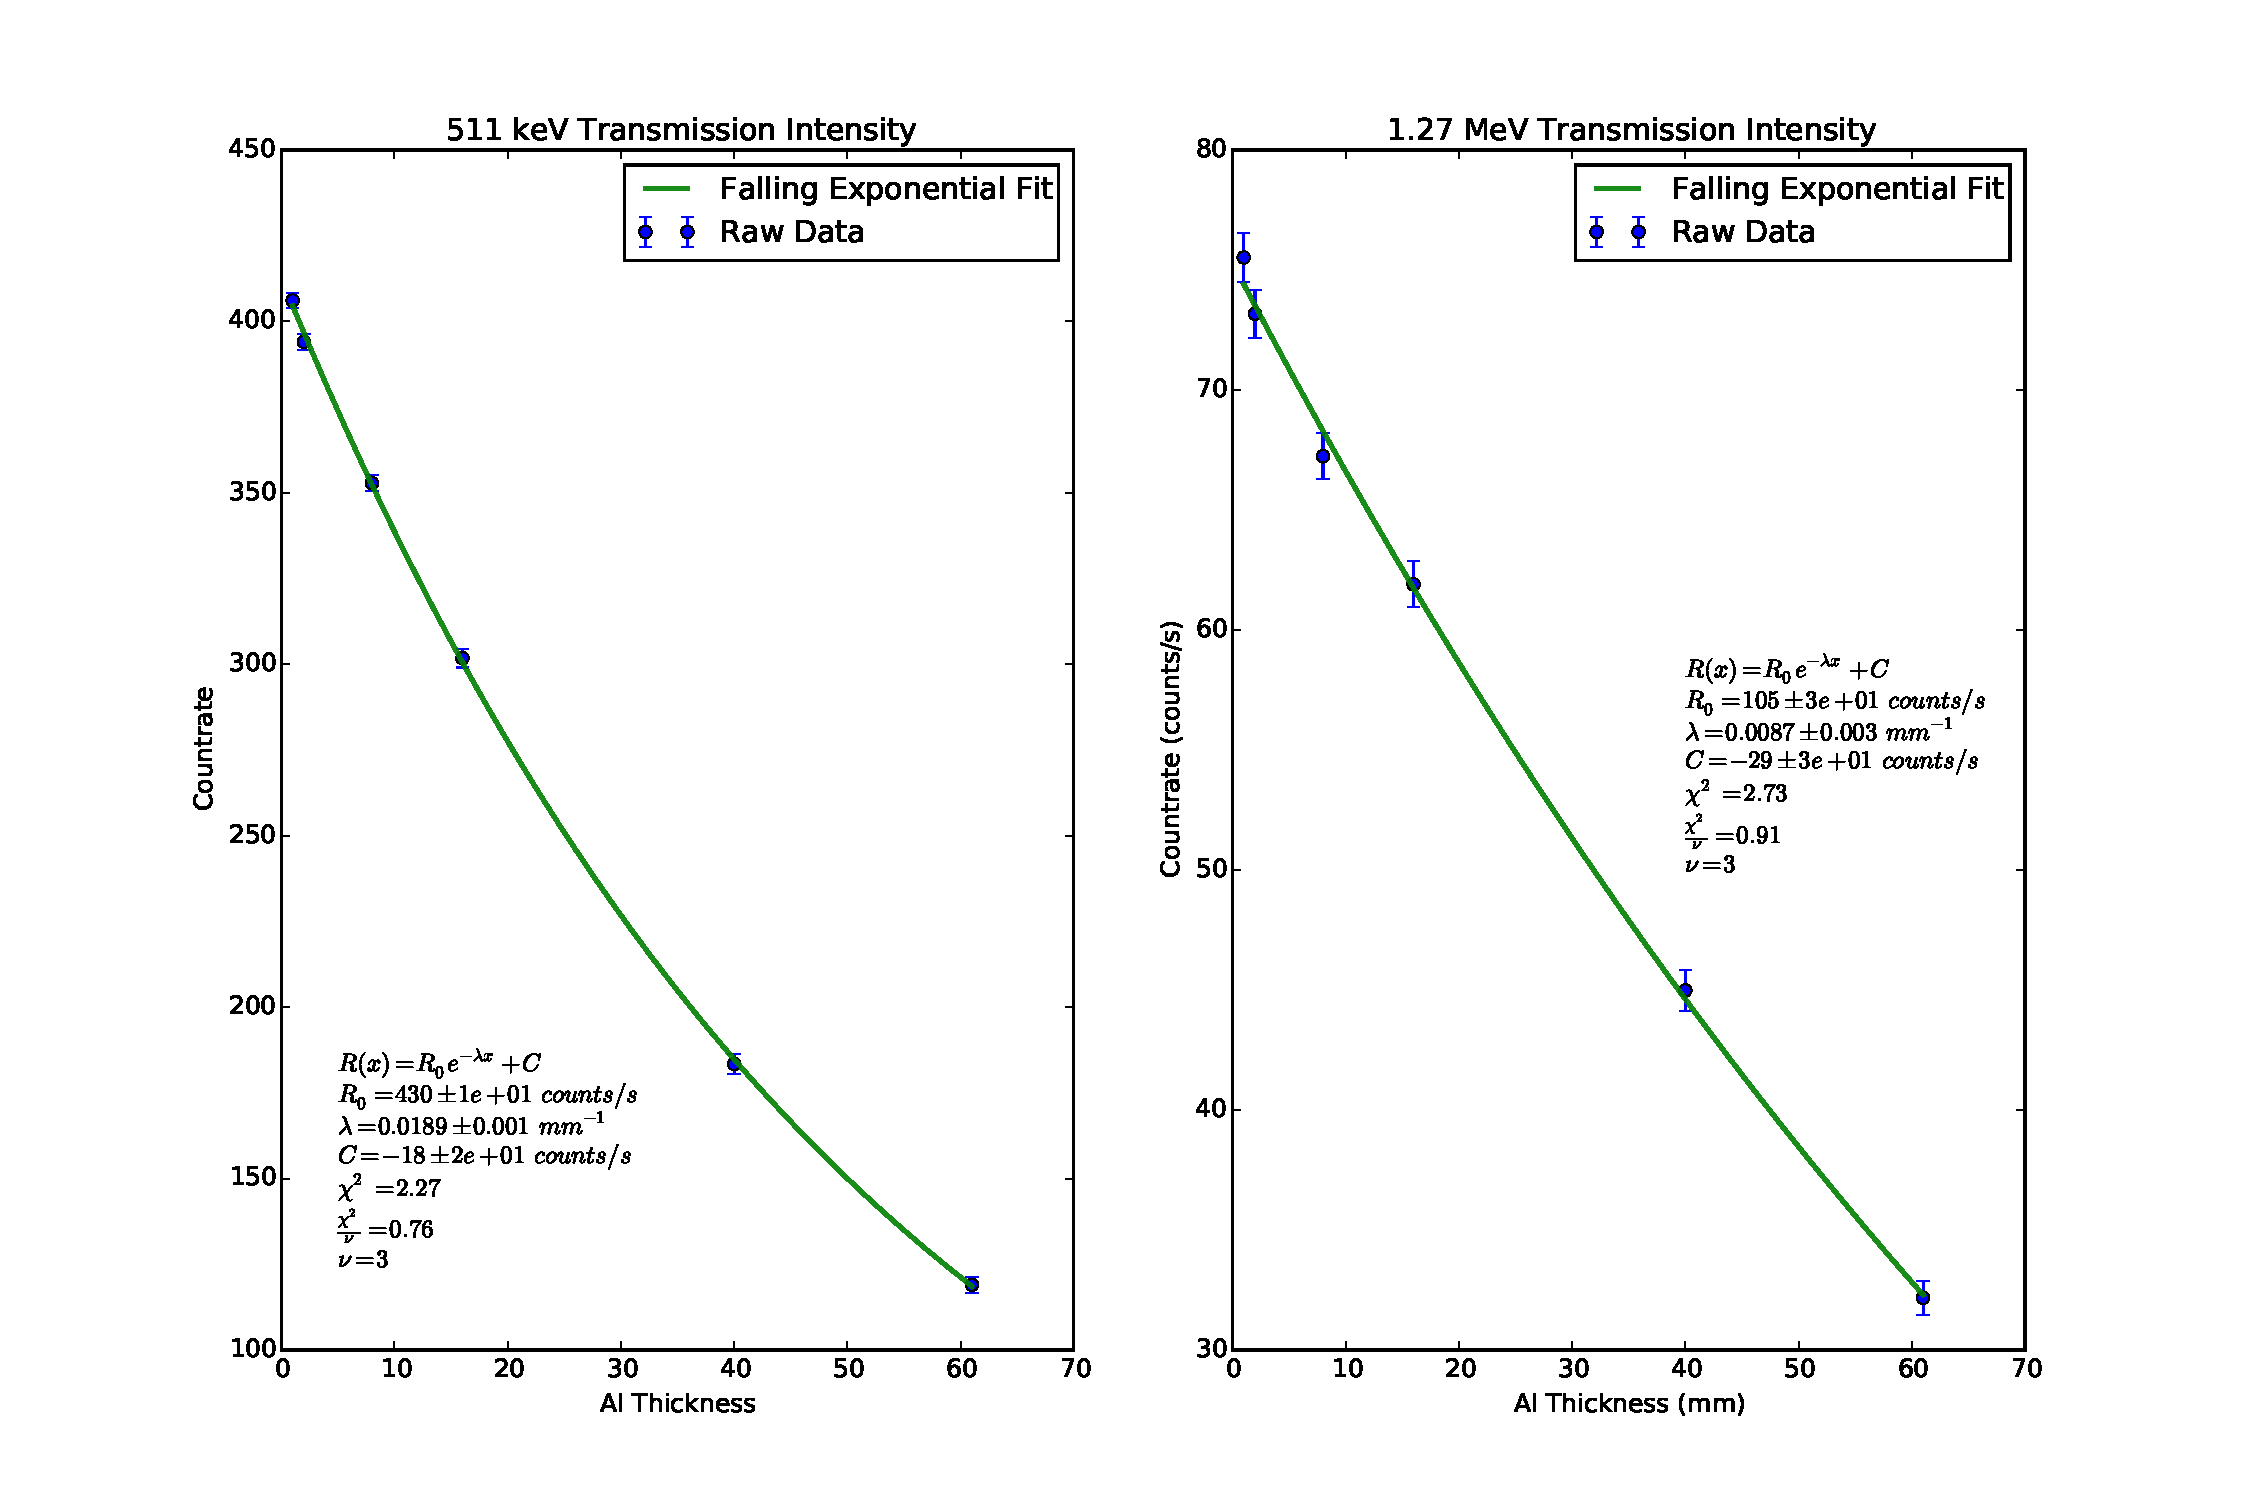
\includegraphics[height=6cm]{../plots/countrates_Na}
		\end{figure}
		Good fits, good agreement with the theory (for the fit at least)
	}
	\frame{
		\frametitle{Fitting to Find Countrates}
		\begin{figure}[!htb]
			\centering
			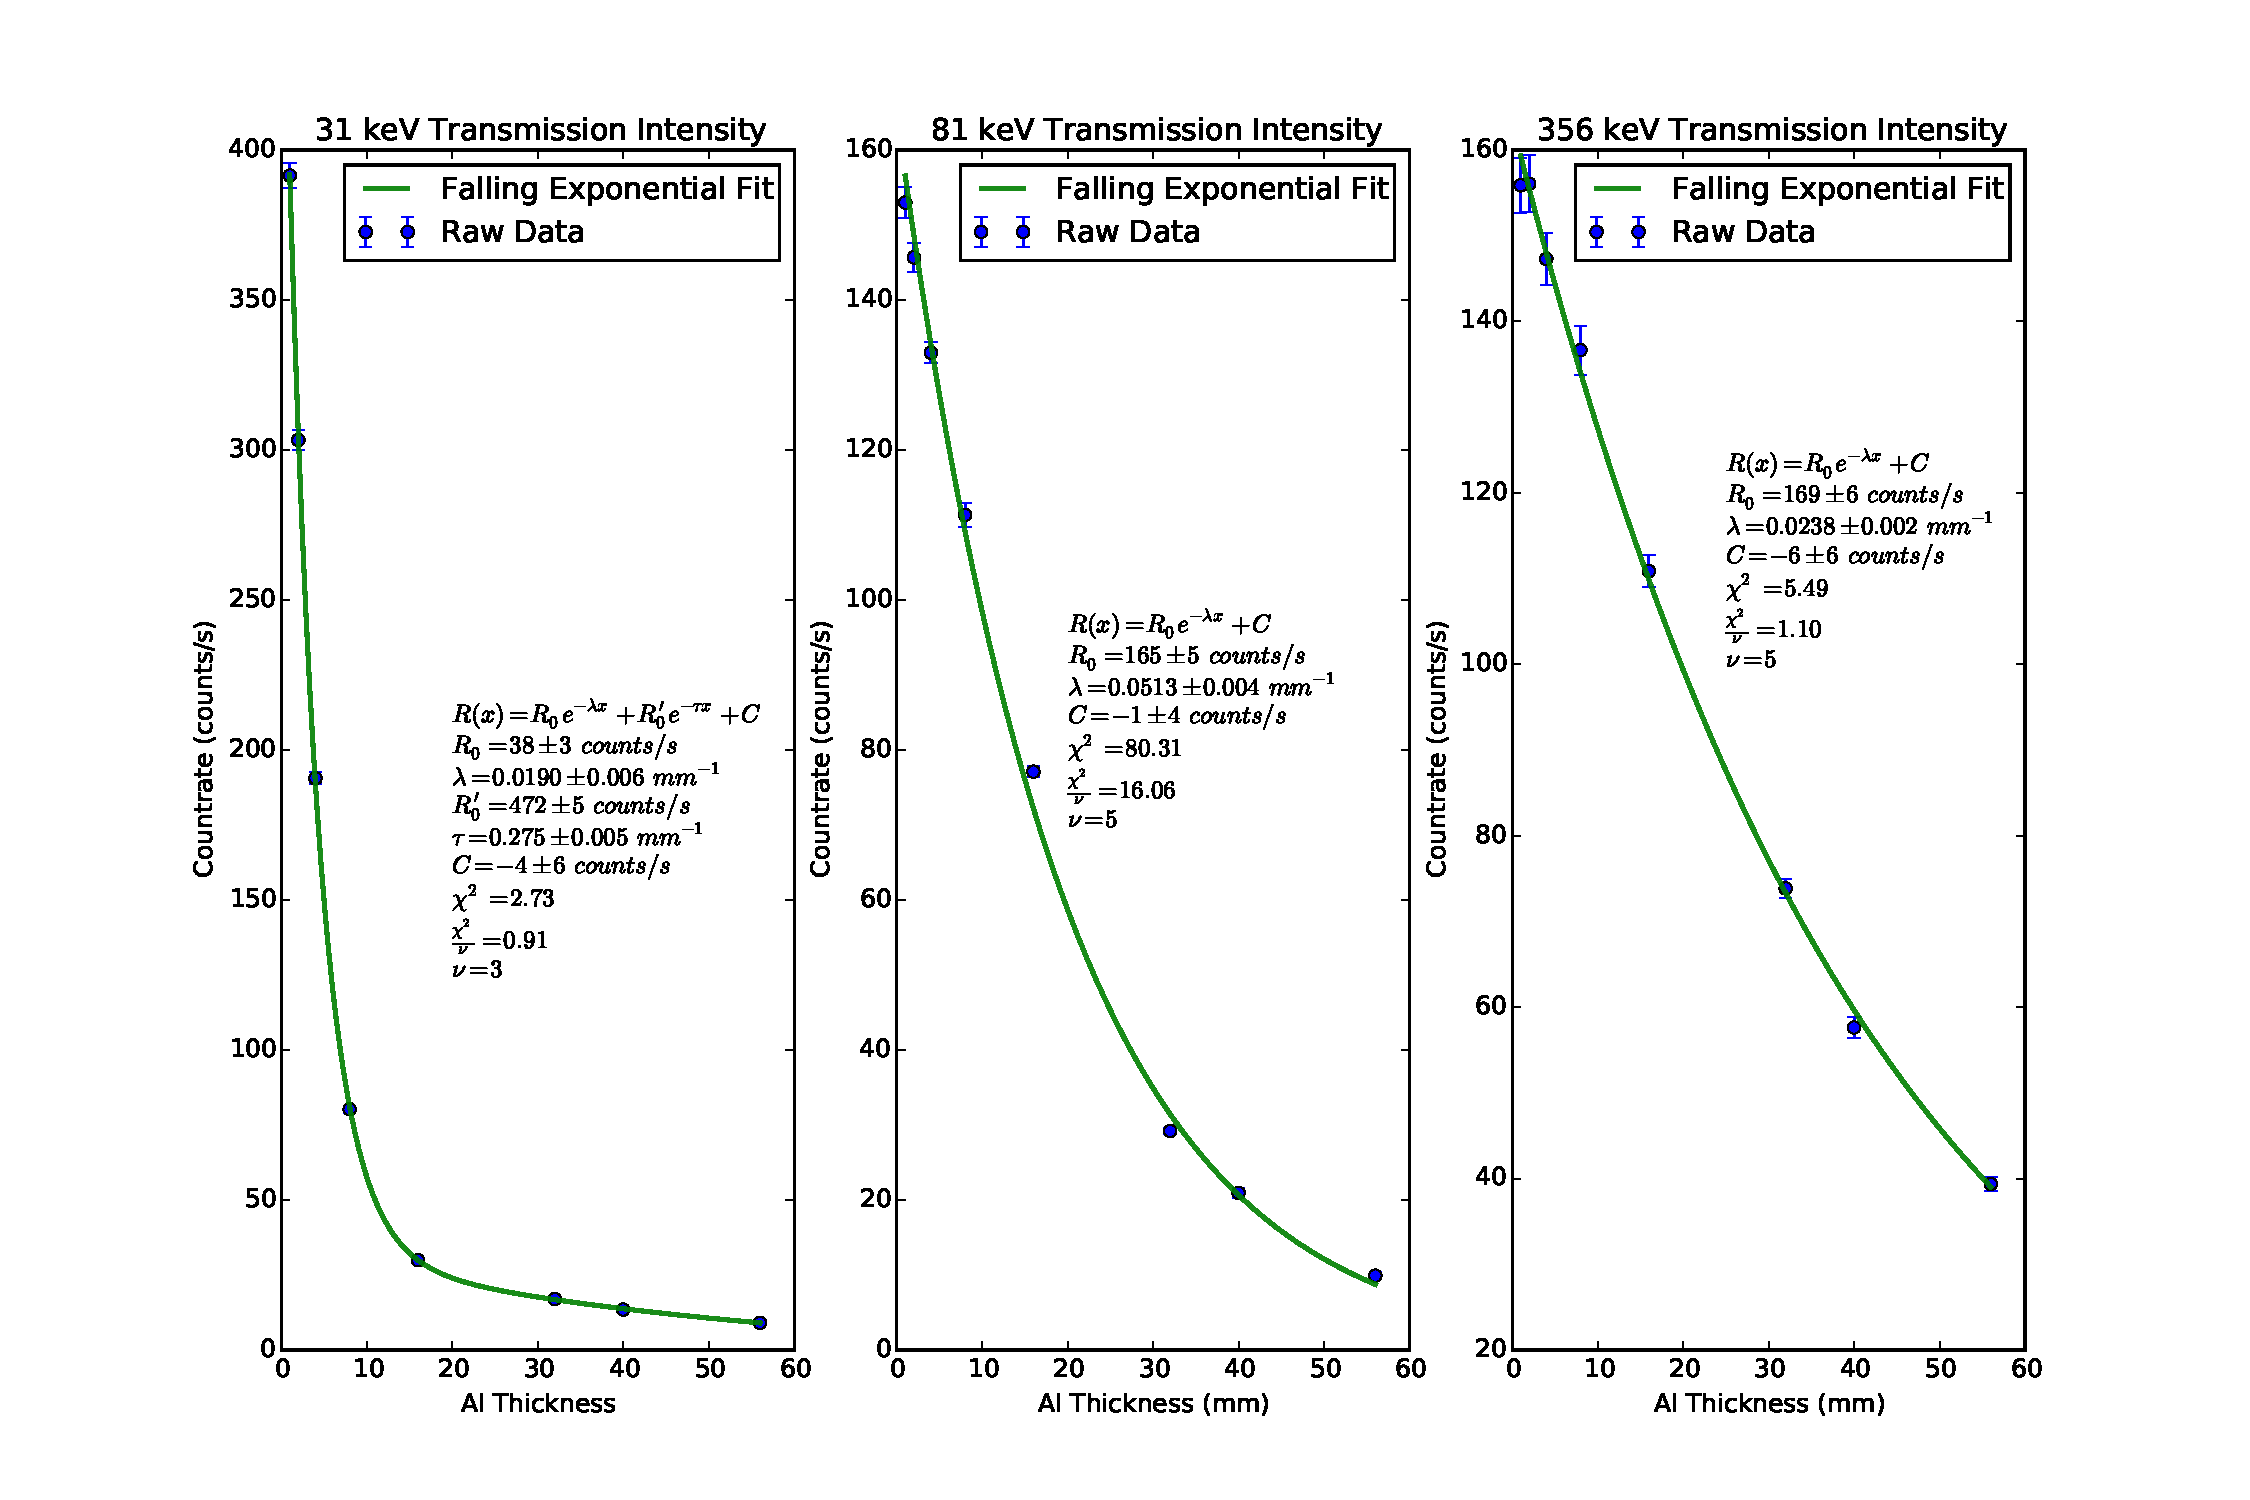
\includegraphics[height=6cm]{../plots/countrates_Ba}
		\end{figure}
		Return to the Ba countrate fits later on
	}

\section{Issues encountered in Analysis}
	\frame{
		\frametitle{How do we stack up?}
		So the Na fit is good, are the values any good?
		$$\mu = \frac{\mu}{\rho} \, x \, \rho = 0.223 cm^{-1}$$
		\begin{flushright}
			\cite{physics.nist.gov}
		\end{flushright}
		Uh oh...
		\begin{gather*}
			\lambda_{exp}\pm\sigma_{\lambda} = 0.19 \pm 0.01 \, cm^{-1}\\
			\sigma_{\lambda} = .01
		\end{gather*}
		$+3\sigma \, \implies$ we either made a discovery or we have a confidence of
		$$100-99.74 = 0.26\%.$$ \cite{taylor}
	}

	\frame{
		\frametitle{How do we stack up?}
		All is not lost, however!  We should test the next measurement.
		$$\mu = \frac{\mu}{\rho} \, x \, \rho = 0.143 cm^{-1}$$
		Hmm, not looking good.
		\begin{gather*}
			\lambda_{exp}\pm\sigma_{\lambda} = 0.09 \pm 0.03 \, cm^{-1}\\
			\sigma_{\lambda} = .03
		\end{gather*}
		$-1.67\sigma \implies$ confidence of 
		$$100-90.5 = 9.5\%$$ \cite{taylor}
		which just tells us we're using student-grade lab equipment in a room of people doing the same experiment.
	}

	\frame[t]{
		\frametitle{Ba Silliness}
		\begin{figure}[!htb]
		\centering
			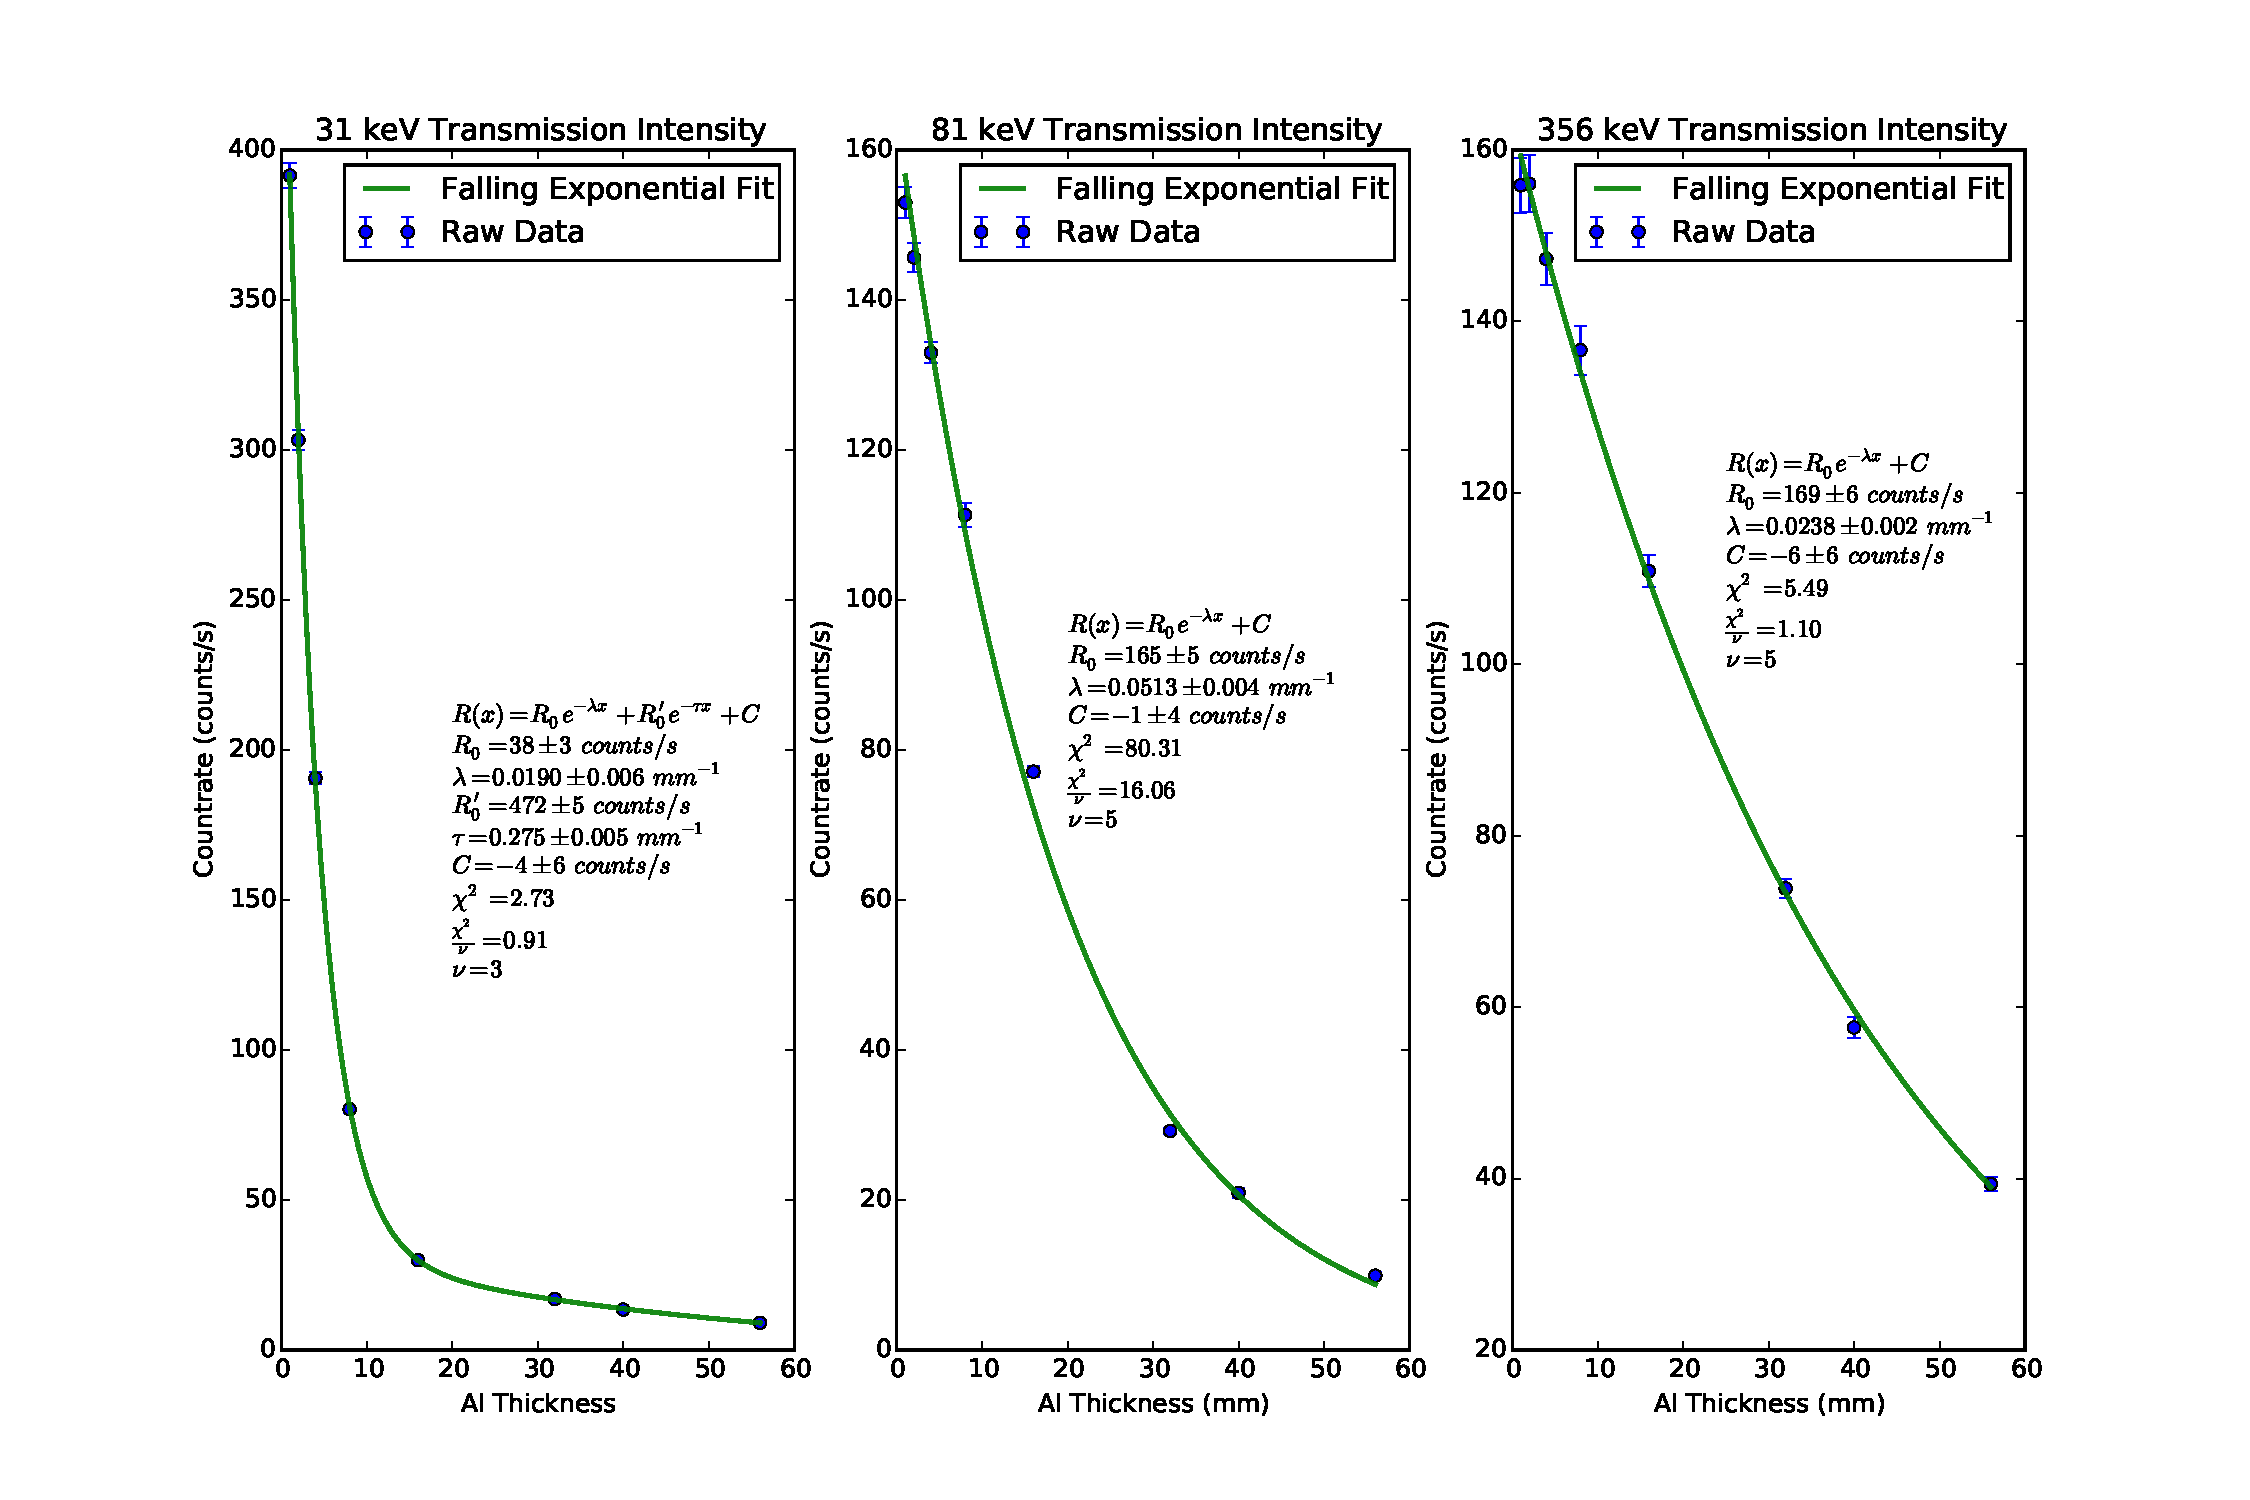
\includegraphics[height=5cm]{../plots/countrates_Ba}
		\end{figure}
		\begin{equation*}
			R(x) = R_0e^{\lambda x} + R_0'e^{\tau x} + C \,~\, 31 \, keV
		\end{equation*}
	}
	\frame{
		\begin{equation*}
			R(x) = R_0e^{\lambda x} + R_0'e^{\tau x} + C
		\end{equation*}
		$R_0e^{\lambda x} + C$ is the normal expression.\\
		\begin{itemize}
			\item Does not account for photoelectric effect dominance at low energies (like 31 keV)!
			\item $\lambda$ = \underline{Compton} effect linear attenuation coefficient
			\item $\tau$ = \underline{Photoelectric} effect linear attenuation coefficient
			\item $\lambda + \tau = 2.94 \, cm^{-1}$
		\end{itemize}
	}
	\frame{
		\frametitle{Ba Silliness}
		So, what's the literature value?
		\begin{gather*}
			\mu = 2.98 \, cm^{-1}\\
			(\lambda+\tau) \pm \sigma_{\tiny{\lambda+\tau}} = 2.94 \pm 0.11 \, cm^{-1}\\
			\implies 0.36\sigma
		\end{gather*}
		Which gives us a confidence value of 
		$$100-28.12 = 71.88\%$$
		in our measurement!\\
		\hspace{1cm}
		\begin{flushleft}
		\tiny{Note that the extra significant figures were added to give a sense of how close the value is, the measurement is properly reported as $2.9\pm0.11 \, cm^{-1}$}
		\end{flushleft}
	}
	\frame{
		\frametitle{And the other energies?}
		Well those are easy.
		\hspace{3cm}
		\begin{center}
		\begin{tabular}{l|c||r}
			$\mu$ & $\lambda\pm\sigma_{\lambda}$ & $\sigma$\\ \hline
			$0.533 \, cm^{-1}$ & $0.51 \pm .04 \, cm^{-1}$ & $0.17\sigma$\\
			$0.260\, cm^{-1}$ & $.23 \pm .02 \, cm^{-1}$ & $0.67\sigma$\\
		\end{tabular}
		\end{center}
	}
	\frame{
		values of lambda are not right on, just best I could find
	}

\section{Resolution}
	\frame{
		other stuff here???
	}
\section{References}
	\frame{
		\frametitle{References}
		\begin{thebibliography}{10}
			\setbeamertemplate{bibliography item}[website]
			\bibitem{physics.nist.gov}
				\small{Physics.NIST.gov - Table of XRay Mass Attenuation Coefficients\\
				http://physics.nist.gov/PhysRefData/XrayMassCoef/ElemTab/z13.html}
			\bibitem{lab manual}
				\small{University of Chicago, PHYS 211 Lab Manual - P211 Wiki}

			\setbeamertemplate{bibliography item}[book]
			\bibitem{taylor}
				\small{An Introduction to Error Analysis - John Taylor}
		\end{thebibliography}
	}

\end{document}
